\chapter{Datasets}

TODO FOR THIS CHAPTER:
\begin{enumerate}
	\item Why we use a constrained time window instead of the whole day
	\item show two sensor location for a dataset (MERL) and discuss the different shapes of the data.  Talk about why it is not necessary to generate results from each location as our datasets already have different shapes and scales of counts
	\item put a marker on the CSMBB sensor we use
	\item put a marker on Denver sensor we use
	\item solve the problem of references subfigures - this CSM latex package is different than other packages I've used before for subfigure reference
	\item discuss the noise in the final datasets
	\item figure out proper name of Denver traffic sensors
\end{enumerate}

This chapter contains information pertaining to the datasets used for our work.  Our datasets are from three different sources.  We have two building datasets and one freeway traffic dataset.  The traffic dataset is a high volume with values taken at 30 minute increments.  The building datasets are much lower volume, but of vastly different types.  One building is a college research and classroom building.  The other is a typical office building.  When considered as a whole, we believe these buildings represent a wide corpus of potential human traffic systems.  All data is scaled to values between 0 and 1.  

\subsection{Building Datasets}
While there has been considerable work in estimating building occupancy values, due to difficulties with acquiring accurate ground truth occupancy values, such datasets are rare.  The problem in acquiring these occupancy values is that many buildings do not have sufficient infrastructure to accurately sense people throughout a building.  One approach used by researchers is to use simulated models of occupancy \cite{page2008, goldstein2010}.  These agent based models have the potential for significant accuracy, but tend not to scale well to large buildings where the large number of agents, rooms and interactions lead to non-trivial solutions.  Due to these problems, for our work, we prefer to estimate occupancy from sensor data rather than simulated data.

To estimate building occupancy from sensor data, numerous techniques have been developed.  A common system uses a combination of simple sensors and wireless motes.  Agarwal, et. al \cite{agarwal2010} created motes using a combination of IR sensors and reed switches placed on doors to determine the likelihood that a room is occupied.  The focus was not on estimating the number of occupants, but instead to determine if the room was occupied at all.  

Mamidi \cite{mamidi2012} and the University of Southern California have developed a building-level energy management system using a combination of motion detectors and environmental sensors to estimate the occupancy of rooms with multiple individuals present.  Ground truth was collected and used as the basis for target values.  These values, coupled with raw sensors were then used to train a machine learning algorithm that was implemented on the motes to estimate occupancy.

Finally, Meyn, et al \cite{meyn2009} created a multiple mote occupancy estimation system using passive infrared sensors, carbon dioxide sensors and coupled this information with building badge counters and video cameras.  In all of the above occupancy estimation system, the researchers were only concerned with estimation and not forecasting.  Also, we were unable to acquire the datasets for testing and due either to the low volume of occupancy or short duration it is likely that the datasets produced by these researchers would not be sufficient for our work.

Our building datasets come from two sources.  The first is a combined research and office building from Mitsubishi's Electronic Research Lab (MERL) dataset \cite{Wren2007}.  The second is a classroom and office building from the Colorado School of Mines (CSMBB) \cite{Hoff2009, Howard2013}.  Both datasets use passive infrared sensors (\ref{fig:pirsensor}) to estimate motion in an area.  

\begin{figure}[h]
	\begin{center}
		\includegraphics[width = .4\linewidth]{pir_sensor}
	\end{center}
	\caption{Passive infrared motion detector}
	\label{fig:pirsensor}
\end{figure}

Due to the nature of IR sensors, we are only able to detect motion instead of actual occupancy; for example, a group of three people would occur as one reading in both systems.  Despite this drawback, real occupancy data would likely be similar to our data, but with higher variance and higher means.  As the range of occupancy estimates in our two datasets are quite different and we are able to achieve accurate estimates in both scenarios, we do not foresee problems when applying our forecasting techniques to more accurate estimated values.  We thus believe this data sufficient to test our occupancy estimation algorithms.

\subsubsection{MERL Dataset} 
The Mitsubishi Electronic Research Labs dataset is derived from a collection of over 200 passive infrared sensors place densely throughout the 7th and 8th floor of a research office building.  This dataset has been used as the basis for multiple areas of research \cite{Wren2003, Wren2006, Wren2007a, Dong2011, Minnen2004, Wren2006a, Wren2007}.  However, none of this research to our knowledge focused on building occupancy forecasting.  The closest related work would be in tracking individuals within the building.

\begin{figure}[!ht]
	\begin{center}
		\subfigure[] {
			\includegraphics[width=0.49\textwidth]{merl_floorplan.png}
			%\label{fig:merl_floor}
		}
		\subfigure[] {
			\includegraphics[width=0.40\textwidth]{merl_map.png}
			%\label{fig:merl_sensors}
		}
	\end{center}
	\caption{Floor plan and sensor locations for the MERL office building dataset.  The red rectangle is the location of our sensor for this work.}
	\label{fig:merlfloor}
\end{figure}

The sensors are placed roughly two meters apart on the ceilings, creating a dense sensing area with little non-sensed space.  Readings are taken at the millisecond level, but due to the sensors' settling times the inter-detection time of motion is approximately 1.5 seconds.  A representation of this floor plan is given in Figure ~\ref{fig:merlfloor}.

The data was collected from March 2006 through March 2008 and there are roughly 53 million sensor readings.  This building is similar to most office buildings with a number of personal offices along with labs and conference rooms.  Employees have roughly set schedules and holidays are observed as normal. 

The counts of sensor activations have been aggregated every 10 minutes.  Because of the lack of significant motion at night, we look only at activations that occur between 6:00am and 7:00pm daily.  A plot of the average activations of all days for a single sensor along with a range of one standard deviation is given in Figure~\ref{fig:merl_day_raw}.

\begin{figure}[!ht]
	\begin{center}
		\subfigure[] {
			\includegraphics[width=0.45\textwidth]{merl_aggregate.png}
		}
		\label{fig:merl_scaled_aggregate}
		\subfigure[] {
			\includegraphics[width=0.45\textwidth]{merl_oneDay.png}
		}
		\label{fig:merl_scaled_raw}
	\end{center}
	\caption{Scaled average readings for a given day and scaled readings for two days from the MERL dataset.}
%	\label{fig:merl_scaled}
\end{figure}

Peak motion unsurprisingly occurs during the middle of the day corresponding to lunch time.  Peak standard deviation appears to occur near noon and 4pm.  The noon variation is unsurprising as people will commonly skip lunch for various reasons.  The 3pm variation is more surprising.  This seems earlier than expected for daily departure, but perhaps it is at the early window of when people will begin to depart for the day.  

As a visual for the typical data values throughout a couple of days is given in Figure~\ref{fig:merl_scaled_aggregate}~\ref{fig:merl_scaled_raw} .  Despite the mean appearing smooth, we see how volatile sensor activation readings are though out the day.


\subsubsection{Colorado School of Mines Dataset}

\begin{figure}[t!]
	\begin{center}
		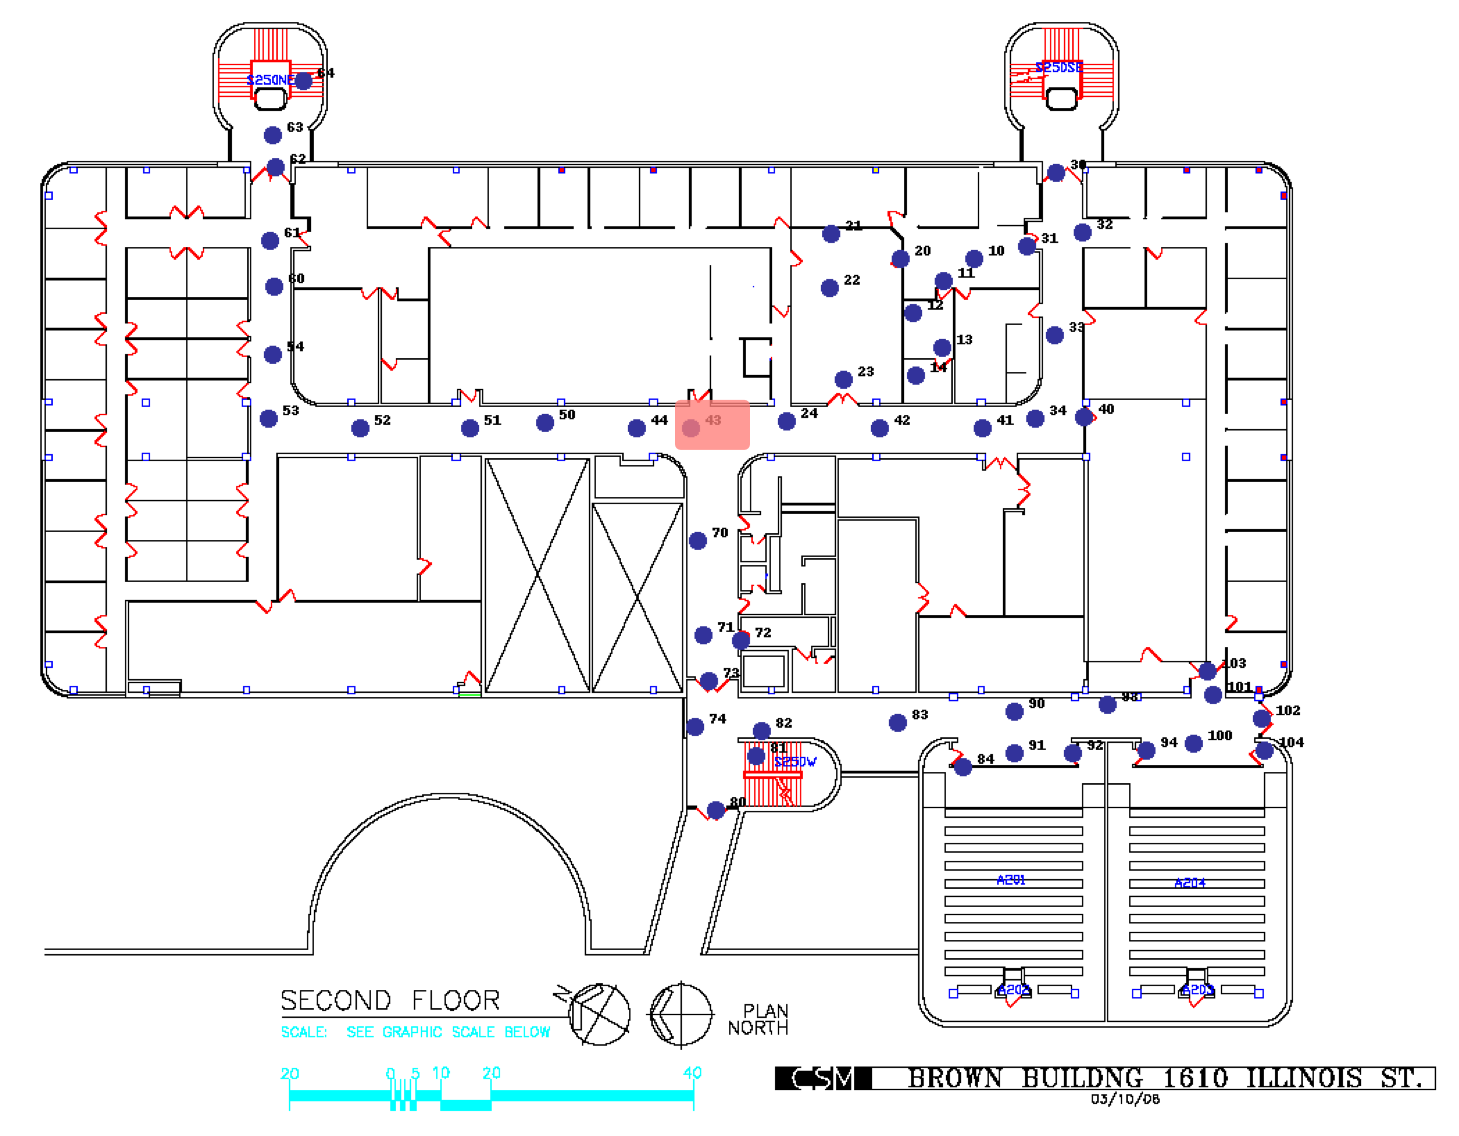
\includegraphics[width=0.5\textwidth]{brown_motes.png}
	\end{center}
	\caption{Sensor locations for the Colorado School of Mines Brown Building}
	\label{fig:csmbbfloor}
\end{figure}

The Colorado School of Mines dataset is a collection of 50 passive infrared sensors mounted on the ceiling of the second floor of a class and office room building.  The density of the sensor placement depends on the location within the building.  Outside the auditorium in the lower right of Figure~\ref{fig:csmbbfloor} is a dense collection of sensors placed approximately every few meters.  Throughout the rest of the building the sensors are placed roughly every 5 meters.  Data was collected for one academic school year from 2008 to 2009 and there are more than 23 million sensor readings.  To acquire readings, the sensors were polled every second and recorded data if motion was detected.  

\begin{figure}[h]
	\begin{center}
		\subfigure[] {
			\includegraphics[width=0.49\textwidth]{brown_day_raw_wed.png}
		}
		\subfigure[] {
			\includegraphics[width=0.49\textwidth]{brown_day_raw_thurs.png}
		}
	\end{center}
	\caption{Average readings from Wednesdays and Thursdays for a given sensor from the MERL dataset.}
	\label{fig:brown_day_raw}
\end{figure}

\ref{fig:brown_day_raw}

This dataset is much different than the MERL dataset as classes typically provide activity on a rigid schedule during the day.  Also as students have exams and projects, late night motion is sporadic based on the time of year.  The counts of sensor activations have been aggregated over every 10 minutes.  Despite occasional late night motion during exam time, most nights have no significant motion.  For this reason we focus on data between 7:00am and 7:00pm daily.  

A plot of the average activations of all Wednesdays and Thursdays for a single sensor along with a range of one standard deviation is given in Figure~\ref{fig:csmday}.  The defined peaks in the dataset correlate to class start and end times when most students will be in the hallways of the building.  Notice how the peak times differ from Wednesday to Thursday.  Classes at the school typically fall into two different schedules; either a class meets on Monday, Wednesday and Friday where the classes are 50 minutes in length or a class meets on Tuesday and Thursday where the classes are 75 minutes in length. 

\begin{figure}[!ht]
	\begin{center}
		\subfigure[] {
			\includegraphics[width=0.45\textwidth]{brown_aggregate.png}
		}
		\label{fig:brown_scaled_aggregate}
		\subfigure[] {
			\includegraphics[width=0.45\textwidth]{brown_oneDay.png}
		}
		\label{fig:brown_scaled_raw}
	\end{center}
	\caption{Scaled average readings for a given day and scaled readings for two days from the CSMBB dataset.}
%	\label{fig:merl_scaled}
\end{figure}

For this work, we focus on the Monday, Wednesday and Friday class schedules.  Figure ~\ref{fig:brown_scaled_aggregate} shows the average of our CSMBB dataset.  Figure ~\ref{fig:brown_scaled_raw} shows a example of raw sensor activations for two days within our CSMBB dataset.


\subsection{Traffic datasets}
Numerous traffic datasets have been used in the time series forecasting literature \cite{Kamarianakis2003, Smith2002, Williams2003, Zhang2009}.  Vehicular traffic datasets are an excellent test for forecasting algorithms as they tend to be highly repetitive with a significant seasonal component.  

\begin{figure}[t!]
	\begin{center}
		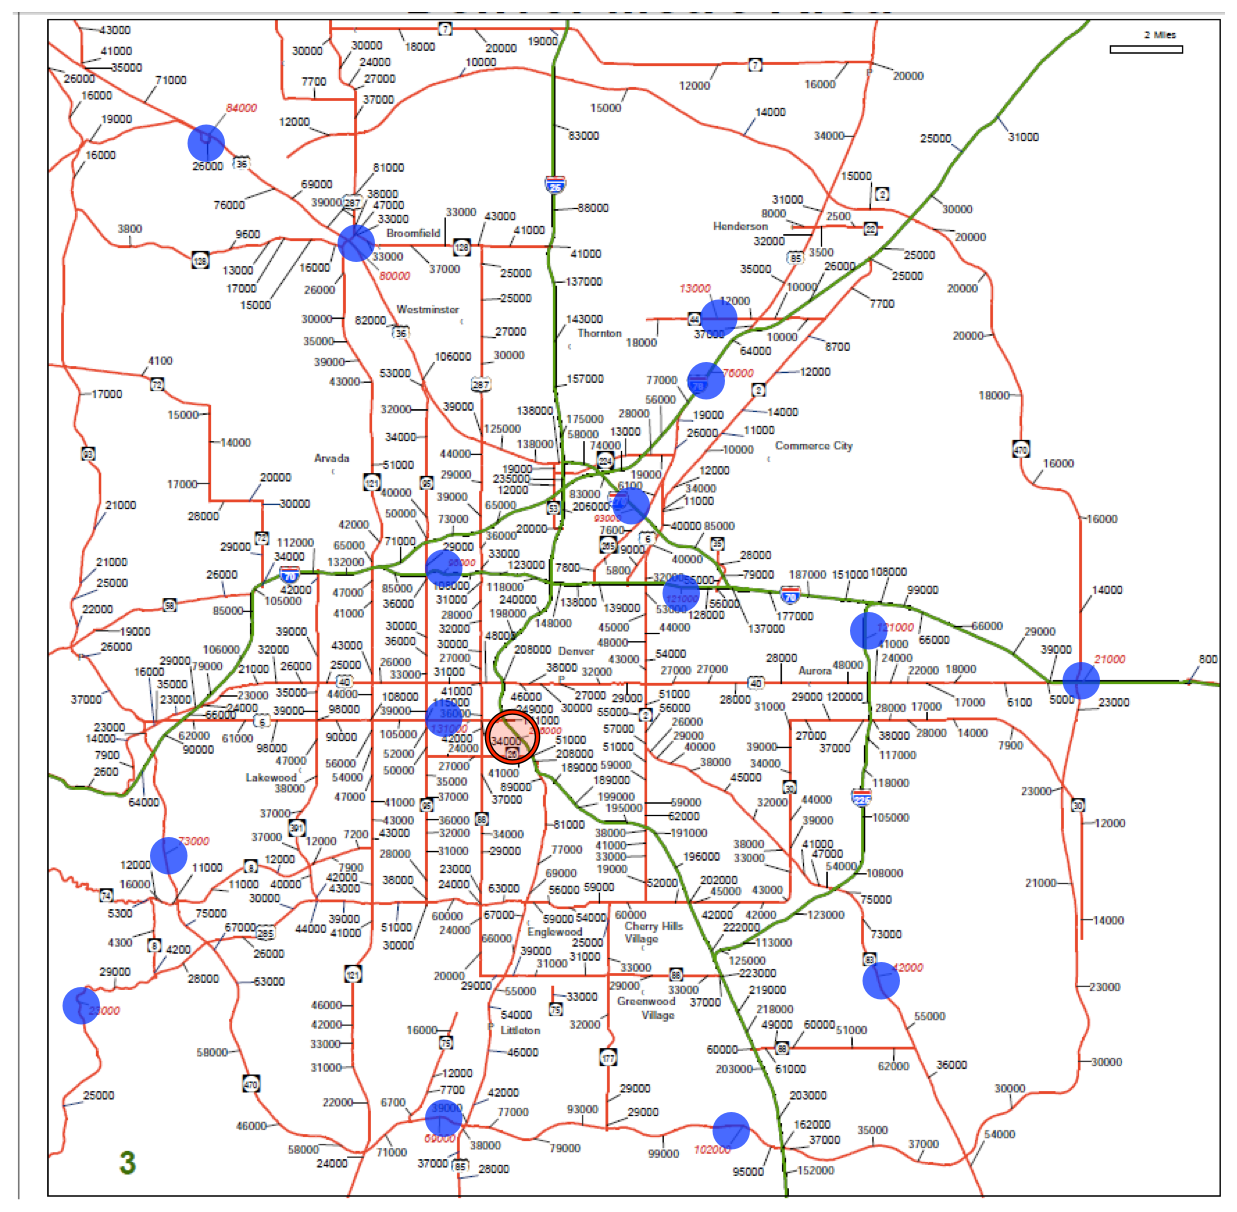
\includegraphics[width=0.5\textwidth]{denver_sensors.png}
	\end{center}
	\caption{City of Denver traffic sensors.}
	\label{fig:denvertraffic}
\end{figure}


\subsubsection{Denver traffic dataset}
The Denver traffic dataset is collected from many in road (TODO FIGURE OUT SENSOR TYPE) sensors which count the number of vehicles passing the sensor throughout the day.  Data is available from 2008 to 2011 on most days of the week.  The data is nearly 1 million readings for the sensors we extracted and approximately 33,000 readings for any one sensor.  For this work we use a freeway sensor near downtown Denver, closely located to Mile High Stadium; the home of the Denver Broncos.  The sensor is located on figure ~\ref{fig:denvertraffic} represented by a red rectangle.

\begin{figure}[h]
	\begin{center}
		\subfigure[] {
			\includegraphics[width=0.49\textwidth]{denver_day_raw_sun.png}
		}
		\subfigure[] {
			\includegraphics[width=0.49\textwidth]{denver_day_raw_mon.png}
		}
	\end{center}
	\caption{Average readings from Sunday and Monday for a given sensor from the Denver traffic dataset.}
	\label{fig:denver_day_raw}
\end{figure}

Count data is aggregated per hour for each direction of traffic at every sensor location.  This data is highly repetitive as Monday through Thursday have approximately the same daily traffic patterns.  Friday behaves much like the rest of the weekdays with the differences being that evening rush hour happens about an hour earlier and their is an increase in night activity.   Example averages for a Sunday and Monday are represented in figure ~\ref{fig:denver_day_raw}.  This figure clearly shows how Monday has a peak time during morning rush hour and a small peak again during afternoon rush hour.  Sunday shows no such pattern.  Instead Sunday shows more slow increase in activity throughout the day.  Also of note is the large amount of sensor activations per hour compared to the CSMBB and MERL datasets.  The counts for Denver traffic are thousands of times larger than our building datasets.

\begin{figure}[h]
	\begin{center}
		\subfigure[] {
			\includegraphics[width=0.45\textwidth]{denver_aggregate.png}
		}
		\label{fig:denver_scaled_aggregate}
		\subfigure[] {
			\includegraphics[width=0.45\textwidth]{denver_oneDay.png}
		}
		\label{fig:denver_scaled_raw}
	\end{center}
	\caption{Scaled average readings for a given day and scaled readings for two days from the Denver traffic dataset.}
%	\label{fig:merl_scaled}
\end{figure}

The scaled dataset that we use for this work is shown in figure \ref{fig:denver_scaled_aggregate}.  This is an average of all Monday through Thursdays for the sensor indicated earlier.  Also, unlike in the other datasets, we do not cut the data down to specific times of day.  This is done, both because there is more traffic during the early morning and late night on this dataset compared to the others and because the data is aggregated only every Hour, do not want to remove more reading from the dataset.  Finally figure \ref{fig:denver_scaled_raw} shows an example of two days of scaled data.  Due to the one hour readings instead of 10 minute readings, the data appears much smoother.  

\subsection{Additional notes on the datasets} 

\noindent
\textbf{Variation in datasets} \\
These three datasets are distinct in many ways.  They differ significantly in total volume of sensor activations, levels of noise in the systems and types of patterns within the datasets.  We believe this variation sufficient to demonstrate the efficacy of our approach to forecasting time series for human controlled environments. \\

\noindent
\textbf{One sensor vs Multiple sensors - why we use a univariate dataset} \\
For this work, we use only one sensor to perform our forecasts.  While intuition may imply that a multivariate approach to forecasting out perform a univariate approach this was show to not be the case by Kamarianakis and Prastacos \ref{kamarianakis2003}.  They studied the problem of forecasting vehicular traffic flow and found similar results using both multivariate and univariate approaches.

We believe the same results hold when it comes to building datasets instead of vehicle datasets.  This is primarily motivated by the simple fact time aggregation and building scale.  For our building datasets, the data is accumulated in 10 minute intervals.  That resolution of detail was empirically selected because it smooths the data sufficiently to allow for accurate forecasting while still being short enough to provide meaningful forecasts.  10 minutes is however, long that it takes an individual to walk from one end of our buildings to the other.  Therefore at a scale of 10 minutes, knowledge of occupancy in one sensor does not seem to imply occupancy in another sensor. \\

\noindent
\textbf{Missing values in the dataset} \\
Due to data collection problems with sensors, the raw data from all of our datasets all had segments with missing values.  These missing values were replace with the historic average value for that sensor at that time on that day.  For example a missing value at 3pm on a Tuesday in the Denver dataset would be replaced by the average value of all Tuesdays at 3pm.




